\providecommand{\main}{../../..}
\documentclass[\main/dresen_thesis.tex]{subfiles}

\begin{document}
  \subsection{BM26B}\label{ch:lss:BM26B}
    \begin{figure}[ht]
      \centering
      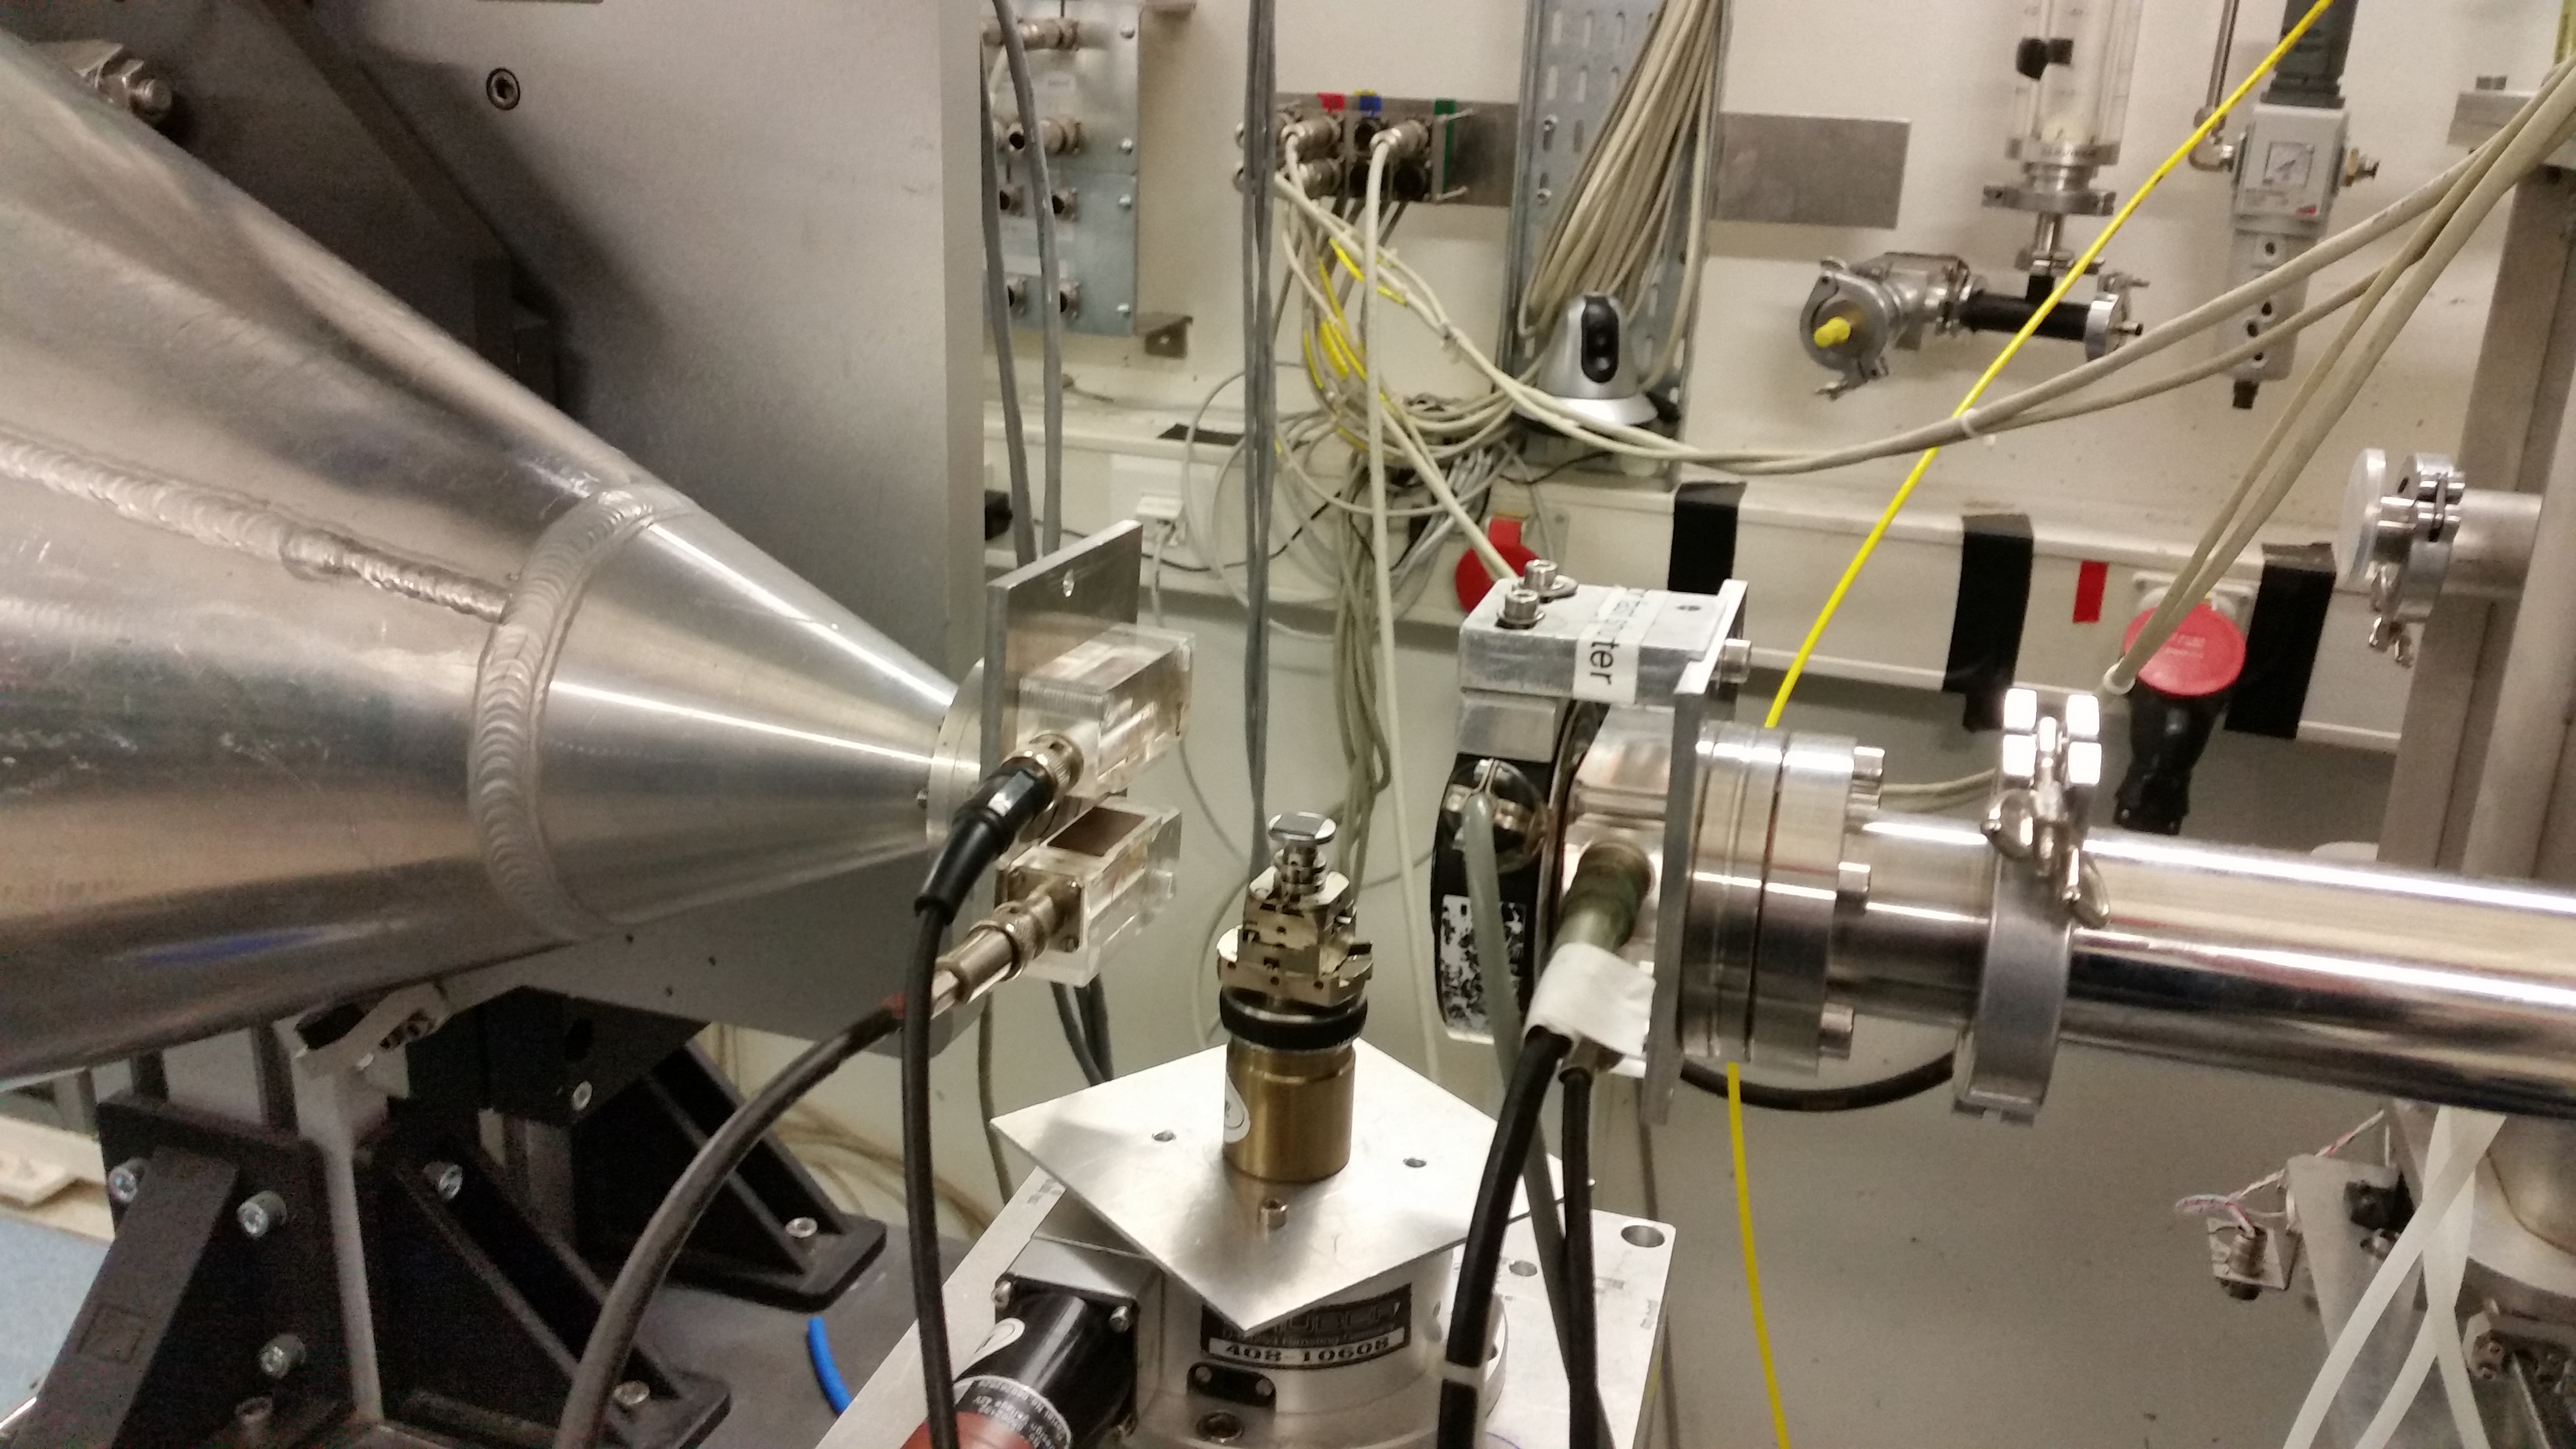
\includegraphics[width=0.7\textwidth]{appendix_instruments_bm26b}
      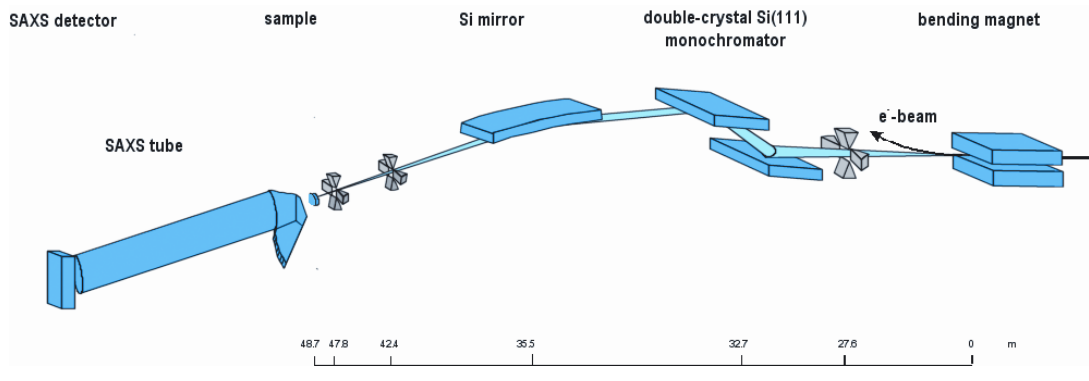
\includegraphics[width=0.7\textwidth]{appendix_instruments_bm26bSetup}
      \caption{\label{fig:lss:BM26B}Sample placement at the BM26B beamline in the ESRF. A high brilliance and collimated X-ray beam (coming from the right) is shined on the sample at a grazing angle, and the scattered intensity is measured on a position-sensitive detector after a evacuated tube of variable length. The beam line schematics are reproduced from \cite{Bras_2003_Recen}.}
    \end{figure}

    The BM26B-Dubble beamline at the European Synchrotron Research Facility is dedicated to SAXS/WAXS measurements and is used in this work for GISAXS experiments.
    The beam line is equipped with a Pilatus 1M detector, equivalent to GALAXI, with an active area of $169 \unit{mm} \times 179 \unit{mm}$ and a pixel size of $172 \unit{\musf m}$.
    It can be placed at a sample-to-detector distance from $1.3 \unit{m}$ up to $7 \unit{m}$.
    At a wavelength of $\lambda \eq 1 \unit{\angstrom}$, the minimum q-value attainable is in the order of $0.028 \unit{nm^{-1}}$, equivalent to a real space $d \eq 225 \unit{nm}$.

    The integrated detector images are obtained in EDF (European Data Format) files, where for each experiment ten measurements are performed at slightly changed detector positions.
    The separate measurements are integrated to obtain a single data set with the gaps removed in between the sensitive areas of the Pilatus 1M detector.
\end{document}